\documentclass[a4paper,
fontsize=11pt,
%headings=small,
oneside,
numbers=noperiodatend,
parskip=half-,
bibliography=totoc,
final
]{scrartcl}

\usepackage{synttree}
\usepackage{graphicx}
\setkeys{Gin}{width=.4\textwidth} %default pics size

\graphicspath{{./plots/}}
\usepackage[ngerman]{babel}
\usepackage[T1]{fontenc}
%\usepackage{amsmath}
\usepackage[utf8x]{inputenc}
\usepackage [hyphens]{url}
\usepackage{booktabs} 
\usepackage[left=2.4cm,right=2.4cm,top=2.3cm,bottom=2cm,includeheadfoot]{geometry}
\usepackage{eurosym}
\usepackage{multirow}
\usepackage[ngerman]{varioref}
\setcapindent{1em}
\renewcommand{\labelitemi}{--}
\usepackage{paralist}
\usepackage{pdfpages}
\usepackage{lscape}
\usepackage{float}
\usepackage{acronym}
\usepackage{eurosym}
\usepackage[babel]{csquotes}
\usepackage{longtable,lscape}
\usepackage{mathpazo}
\usepackage[flushmargin,ragged]{footmisc} % left align footnote

\usepackage{listings}

\urlstyle{same}  % don't use monospace font for urls

\usepackage[fleqn]{amsmath}

%adjust fontsize for part

\usepackage{sectsty}
\partfont{\large}

%Das BibTeX-Zeichen mit \BibTeX setzen:
\def\symbol#1{\char #1\relax}
\def\bsl{{\tt\symbol{'134}}}
\def\BibTeX{{\rm B\kern-.05em{\sc i\kern-.025em b}\kern-.08em
    T\kern-.1667em\lower.7ex\hbox{E}\kern-.125emX}}

\usepackage{fancyhdr}
\fancyhf{}
\pagestyle{fancyplain}
\fancyhead[R]{\thepage}

%meta
%meta

\fancyhead[L]{G. Schifferdecker \\ %author
LIBREAS. Library Ideas, 26 (2014). % journal, issue, volume.
\href{http://nbn-resolving.de/urn:nbn:de:kobv:11-100222640
}{urn:nbn:de:kobv:11-100222640}} % urn
\fancyhead[R]{\thepage} %page number
\fancyfoot[L] {\textit{Creative Commons BY 3.0}} %licence
\fancyfoot[R] {\textit{ISSN: 1860-7950}}

\title{\LARGE{WWC - WeberWorldCafé. Ein Interview}} %title %title
\author{Gesche Schifferdecker} %author

\setcounter{page}{72}

\usepackage[colorlinks, linkcolor=black,citecolor=black, urlcolor=blue,
breaklinks= true]{hyperref}

\date{}
\begin{document}

\maketitle
\thispagestyle{fancyplain} 

%abstracts

%body
\emph{LIBREAS}: Liebe Gesche Schifferdecker, Sie sind Referentin für
Öffentlichkeitsarbeit mit dem Schwerpunkt Online-Kommunikation bei der
Max Weber Stiftung, betreuen redaktionell zahlreiche Wissenschaftsblogs
und organisieren zudem die Veranstaltungsreihe \enquote{WeberWorldCafé}.

\section*{Schwerpunkt Konzept und
Ablauf}\label{schwerpunkt-konzept-und-ablauf}

\emph{LIBREAS}: Wie sind Sie mit diesem Veranstaltungsformat in
Berührung gekommen? Und erschien es Ihnen gleich relevant für die
Anwendung in der Max Weber Stiftung? Brauchte es besondere
konzeptionelle Anpassungen?

\emph{Gesche Schifferdecker}: Wir führen die WeberWorldCafés im Rahmen
eines Verbundprojektes mit dem Forum Transregionale Studien durch, das
vom Bundesministerium für Bildung und Forschung (BMBF) gefördert wird.
Die Idee hinter den WeberWorldCafés ist, neue, jüngere Zielgruppen aus
SchülerInnen, Studierenden und Young Professionals zu erschließen, die
gegebenenfalls nicht zu unseren Konferenzen, Paneldiskussionen oder
Vorträgen kommen (würden). Deswegen haben wir das World Café als
interaktives Format gewählt, das jüngere Menschen anspricht.
Gleichzeitig geht es uns um die Internationalisierung der Geistes- und
Sozialwissenschaften. Diese erreichen wir, indem wir
WissenschaftlerInnen aus den Instituten der Max Weber Stiftung und
Fellows des Forums mit anderen WissenschaftlerInnen, Studierenden und
Laien aus der ganzen Welt in Deutschland zusammenbringen. Ein mögliches
Veranstaltungsformat wäre hier aber auch zum Beispiel ein BarCamp
gewesen. Konzeptionelle Anpassungen brauchten wir insofern, als dass
beim World Café ursprünglich keine ExpertInnen vorgesehen sind. Wenn man
allerdings zu wissenschaftlichen Themen arbeitet, ist es sinnvoll,
WissenschaftlerInnen als sogenannte \enquote{TischgastgeberInnen}
einzuladen, die zumindest in die Thematik einführen und das Gespräch bei
Bedarf lenken. Dabei ist es aber nicht das Ziel, dass die
TischgastgeberInnen einen Vortrag halten. Alle GesprächsteilnehmerInnen
sind gleichberechtigt und sollen sich in die Diskussion mit einbringen.
Dies beinhaltet auch, dass zum Beispiel eine deutsche Politikprofessorin
einer ukrainischen Bloggerin aufmerksam zuhört, und dass eine iranische
Nachwuchsjournalistin einer Wissenschaftlerin, die im Libanon forscht,
ihre persönliche Einschätzung zur Iran-Syrien-Achse darlegt. Allerdings
haben wir die Erfahrung gemacht, dass die TeilnehmerInnen anfangs recht
schüchtern und deswegen dankbar sind, wenn eine Expertin bzw. ein
Experte das Gespräch beginnt.

\begin{figure}[htbp]
\centering
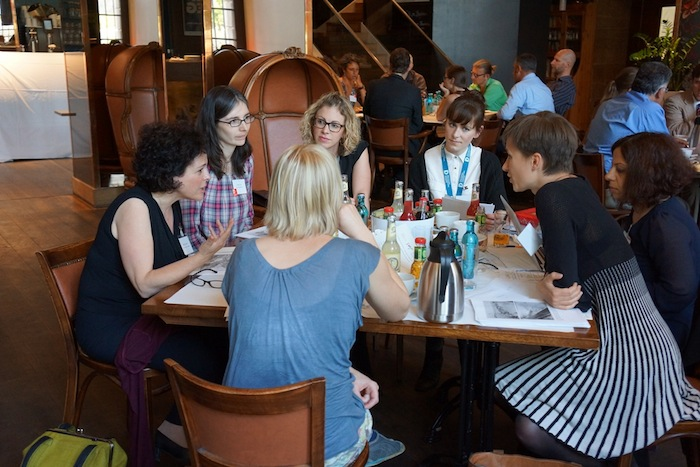
\includegraphics{wwc1.jpg}
\caption{WeberWorldCafé 2014}
\end{figure}

\emph{LIBREAS}: Wie wählen Sie Experten für Ihr WeberWorldCafé (WWC)
aus? Wer gilt dabei als Experte?

\emph{Gesche Schifferdecker}: Wer als ExpertIn gilt, hängt stark vom
Thema ab. Beim ersten WeberWorldCafé zum Thema \enquote{Bürger, Blogger,
Botschafter: Neue Medien und Akteure in der Diplomatie des 21.
Jahrhunderts} (\url{http://trafo.hypotheses.org/738}) ging es uns zum
Beispiel darum, nicht nur mit Politik- und MedienwissenschaftlerInnen
sowie mit HistorikerInnen zu diskutieren, sondern auch die Perspektive
der praktischen Diplomatie abzubilden. Deswegen haben wir einen
ägyptischen Blogger, einen Vertreter der Deutschen Welle und einen des
Goethe-Instituts und die Leiterin des \enquote{Diplomatenkollegs} für
nichtdeutsche Diplomaten im Auswärtigen Amt eingeladen. Es war eine
bunte Mischung. Vor dem Hintergrund, dass die WeberWorldCafés im Rahmen
unseres Verbundprojekts mit dem Forum Transregionale Studien
durchgeführt werden, ist es uns natürlich auch wichtig,
WissenschaftlerInnen aus den Auslandsinstituten der Max Weber Stiftung
und Fellows des Forums als TischgastgeberInnen miteinzubeziehen, die zu
bestimmten Schwerpunkten arbeiten, und diese zusammenzubringen. Diese
Prämisse beeinflusst auch die Themenwahl. Weiterhin achten wir darauf,
hauptsächlich NachwuchswissenschaftlerInnen auszuwählen -- zum einen vor
dem Hintergrund, dass die Förderung des akademischen Nachwuchses zu den
wichtigsten Zielen des Verbundprojektes der Max Weber Stiftung und des
Forum Transregionale Studien gehört, und zum anderen, weil jüngere
WissenschaftlerInnen häufig offener für neue, interaktive Formate sind.
Trotzdem ist eine der ersten Fragen der TischgastgeberInnen meistens, ob
sie ein Paper oder eine Präsentation vorbereiten sollen. Wenn sie dann
erfahren, dass es \enquote{nur} um den Wissensaustausch und die
Diskussion vor Ort geht, ist die Verwunderung groß. Diese Reaktion
zeigt, wie stark bereits NachwuchswissenschaftlerInnen in den
klassischen Veranstaltungs- und Publikationsstrukturen verhaftet sind.
Viele haben auch besonderen Respekt vor dem direkten Kontakt mit
fachfremdem Publikum -- aber niemand hat bis jetzt wegen des Formats
nicht teilnehmen wollen. Vielmehr haben mir einige TischgastgeberInnen
gesagt, dass sie gerade wegen dieser neuen Herausforderung zugesagt
hätten.

\emph{LIBREAS}: Wie geht das WWC mit den Resultaten um? Gab es bei den
vergangenen Veranstaltungen Nachbereitungen und wenn ja welcher Art?
Welche Folgeprojekte, -diskussionen oder -sichtweisen kamen eventuell
zustande?

\emph{Gesche Schifferdecker}: Sinn und Zweck des WeberWorldCafés ist
eigentlich der Workshop an sich, das heißt der Austausch vor Ort.
Allerdings hat es uns, als wir das erste WeberWorldCafé planten, nicht
gefallen, dass das Format nicht vorsieht, dass die Resultate der
Diskussionen veröffentlicht werden. So haben wir uns entschlossen, über
Twitter und unsere verschiedenen Blogs sogenannte
\enquote{Science-ReporterInnen} zu suchen, deren originäre Aufgabe es
ist, die Diskussionen, Prozesse und Ergebnisse der Tische
zusammenzufassen und eine Art Reportage darüber zu schreiben. Diese
Beiträge werden dann entweder auf den Blogs der ReporterInnen oder auf
unserem WWC-Blog veröffentlicht (zum Beispiel
\url{http://wwc.hypotheses.org/187} und
\url{http://wwc.hypotheses.org/498}). Zur Nachbereitung gehörte auch
jeweils ein Twitter-Storify, mit dessen Hilfe die punktuellen Eindrücke
der Twitter-affinen TeilnehmerInnen über einen Hashtag nachvollzogen
werden konnten.

Ebenso wichtig wie die Nachbereitung finde ich aber auch die
Vorbereitung der Events, die wir über unser WWC-Blog
(\url{http://wwc.hypotheses.org/}) intensiv betreiben: Wir führen
Interviews mit einigen TischgastgeberInnen und stellen diese vor, posten
thematisch passende Beiträge und geben Tipps zur Vorbereitung der
WeberWorldCafés. Auf dem Blog findet demzufolge auch eine umfang- und
facettenreiche Veranstaltungsdokumentation statt.

\emph{LIBREAS}: WorldCafés eignen sich ja eher für breitere Themen, so
Ihre These in Ihrem Artikel in der MusErMeKu
(\url{http://musermeku.hypotheses.org/1781}). Bei dem jüngsten
WeberWorldCafé im September haben Sie den Themenkreis spezifiziert. Hat
sich das WorldCafé trotzdem geeignet oder stößt es bei einem konkreteren
Thema eher auf seine Grenzen?

\emph{Gesche Schifferdecker}: Die Planung unseres WeberWorldCafés im
September 2014 zum Thema \enquote{Narrating the First World War --
Experiences and Reports from Transregional Perspectives}
(\url{http://wwc.hypotheses.org/302}) war tatsächlich eine
Herausforderung! Wir haben uns gefragt: Welche Fragen hat unsere
Zielgruppe an den Ersten Weltkrieg? Welche Perspektiven sind interessant
und wurden im öffentlichen Diskurs noch kaum beachtet? Was sagt der
Erste Weltkrieg jungen Menschen heute? Wie kann er erfahrbar gemacht
werden? Unser Vorteil war, dass der Erste Weltkrieg bisher hauptsächlich
in nationalen Kontexten dargestellt und diskutiert worden ist. Insofern
war unser Ansatz, über die regionalen Tische quasi einen
\enquote{Weltblick} zu ermöglichen, innovativ und für unser WWC-Format,
bei dem es vier Runden gibt und nach etwa 25 Minuten die Tische
gewechselt werden müssen, durchaus geeignet. Intensiv beschäftigt hat
uns allerdings die Frage, wie wir einen Diskurs zwischen
WissenschaftlerInnen aus der ganzen Welt, die zu unterschiedlichen
Regionen und zu unterschiedlichen Perspektiven auf den Ersten Weltkrieg
forschen, und Laien initiieren können. Gleichzeitig haben wir damit
gerechnet, dass zusätzlich zu den interessierten fachfremden
TeilnehmerInnen auch zahlreiche HistorikerInnen, die zum Ersten
Weltkrieg forschen, am WeberWorldCafé teilnehmen werden. Wie sollte man
diese sehr unterschiedlichen Erfahrungshorizonte und Kenntnisse nun
unter einen Hut bekommen? Im Rahmen dieser Überlegungen kam uns dann die
Idee, an den Tischen mit Quellen, das heißt Briefen, Fotos, Landkarten,
Zeitzeugenberichten et cetera zu arbeiten, mit dem Ziel, den Ersten
Weltkrieg \enquote{erfahrbar} zu machen. Gleichzeitig bot das
WeberWorldCafé allen TeilnehmerInnen die Möglichkeit, Fragen jeglicher
Art zu stellen, die man zum Beispiel nach einem Vortrag niemals stellen
würde. Diese Chance haben alle TeilnehmerInnen, ob Mathematik- oder
Architekturstudent, Kuratorin, Doktorandin der Geschichtswissenschaft
oder Stiftungsmitarbeiterin, genutzt. Und so wurden auch die
WissenschaftlerInnen, die seit vielen Jahren zum Ersten Weltkrieg
forschen, durch die Fragen der TeilnehmerInnen und deren an anderen
Tischen gewonnenen Perspektiven auf andere Regionen mit neuen
Blickwinkeln konfrontiert. Ein Beispiel hierfür ist: Die Gründe, warum
die ostafrikanischen Askari für das Deutsche Reich in den Krieg zogen,
waren andere als jene der australischen Aborigines. Der Umgang mit den
Ureinwohnern nach dem Krieg allerdings war in Ostafrika und Australien
sehr ähnlich. Damit hatten sich bis dahin weder die Tischgastgeber des
Afrika-Tischs noch die Wissenschaftlerin, die über Australiens Rolle im
Ersten Weltkrieg forscht, auseinandergesetzt.

\section*{Schwerpunkt Kreativität und
Dialog}\label{schwerpunkt-kreativituxe4t-und-dialog}

\emph{LIBREAS}: Wodurch kann die Kreativität, die, wie Sie in Ihrem
Artikel in der MusErMeKu schreiben, unerwartete Perspektiven eröffnet
und zu erstaunlichen Verbindungen führt, gefördert werden? Und warum ist
kreatives Denken so wichtig für den eigentlich ja sehr formalisiert
ablaufenden wissenschaftlichen Diskurs?

\emph{Gesche Schifferdecker}: Die Perspektiven sind in erster Linie
unerwartet, weil die TeilnehmerInnen bisher nicht ausgesucht wurden,
sondern sich bei beiden WeberWorldCafé jeweils anders zusammensetzen. So
kommen unterschiedliche Disziplinen zusammen, unterschiedliche
berufliche Hintergründe, unterschiedliche Generationen -- denn obwohl
das WWC zwar eine jüngere Zielgruppe hat, schließen wir andere
Interessierte natürlich nicht aus. Gefördert werden die
Austauschprozesse durch das Format, das alle Beteiligten quasi zwingt,
mitzudenken und sich einzubringen. Für die TischgastgeberInnen bedeutet
das, \enquote{outside of the box} zu denken, mit Menschen konfrontiert
zu werden, die ihnen Fragen stellen, die sie von den FachkollegInnen
nicht gefragt werden.

\begin{figure}[htbp]
\centering
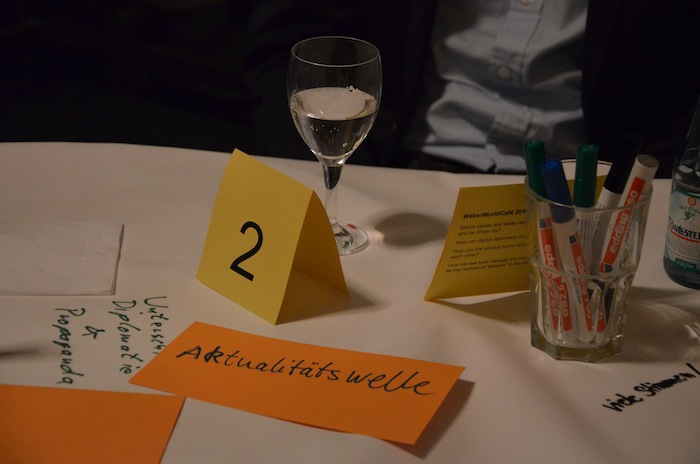
\includegraphics{wwc2.jpg}
\caption{WeberWorldCafé 2014}
\end{figure}

\emph{LIBREAS}: Könnte das WeberWorldCafé die Funktion einer bisherigen
Konferenz als Austauschformat in der Wissenschaftskommunikation
maßgeblich ergänzen oder sogar ablösen?

\emph{Gesche Schifferdecker}: Nein, das glaube ich nicht und das würde
ich mir auch nicht wünschen. Ich finde es wichtig, dass verschiedene
Formate nebeneinander existieren. Die Konferenz dient eher dem
wissenschaftlichen Austausch mit KollegInnen, während es bei den
WeberWorldCafés um einen Dialog mit einem sehr unterschiedlich
zusammengesetzten Publikum geht. Hinzu kommt, dass die
TischgastgeberInnen an ihren Tischen bleiben und sich dementsprechend
mit den anderen ExpertInnen während des Cafés nicht austauschen. Man
kann die Formate deshalb nicht miteinander vergleichen.

\section*{Schwerpunkt Anwendung}\label{schwerpunkt-anwendung}

\emph{LIBREAS}: Welchen Stellenwert hat das WeberWorldCafé bereits für
den Diskurs innerhalb der Geschichtswissenschaft oder
Geisteswissenschaften?

\emph{Gesche Schifferdecker}: Während das Format zum Beispiel im Bereich
der Weiterbildungsbranche schon fast ein \enquote{alter Hut} ist, ist es
für die meisten Geistes- und Sozialwissenschaftler neu. Aber einige der
TeilnehmerInnen waren sehr angetan und planen, World Cafés auch
innerhalb ihrer Organisationen durchzuführen. Im Bereich der
Geschichtswissenschaft fände ich dies besonders reizvoll, da das
WeberWorldCafé durch den interdisziplinären und transregionalen
Austausch die Möglichkeit bietet, bestimmte Ereignisse mit dem Ansatz
der sogenannten \enquote{Histoire croisée} zu betrachten, also aus dem
Blickwinkel einer multiperspektivischen transnationalen
Geschichtsschreibung. Ich bin gespannt, ob sich dieses Format etablieren
wird.

\emph{LIBREAS}: Wenn andere Disziplinen ein solches Veranstaltungsformat
organisieren wollten, welchen Rat würden Sie geben, worauf besonders bei
der Vorbereitung geachtet werden müsste?

\emph{Gesche Schifferdecker}: Ich kann nicht beurteilen, ob sich das
World Café als Format überhaupt für alle Wissenschaftsdisziplinen
eignet. Ich kenne die Kommunikationsstrukturen in einigen Fächern nicht,
beispielsweise in der Mathematik oder in der Computerlinguistik. In den
Geistes- und Sozialwissenschaften sowie den Rechts- und
Lebenswissenschaften -- also in allen Disziplinen, in denen über Fakten
hinaus verschiedene Sichtweisen ausgetauscht werden -- ist es aber
sicherlich sinnvoll, World Cafés zu veranstalten. Man könnte diese in
unserem Stil, das heißt mit ExpertInnen als TischgastgeberInnen
organisieren, aber auch beispielsweise Studierende eines Fachs oder
DoktorandInnen zu einem spezifischen Thema miteinander in einen Dialog
bringen, ohne dass es eine Person am Tisch gibt, die \enquote{mehr weiß}
als die anderen und auf dieser Basis das Gespräch gegebenenfalls leicht
steuert. Wenn man allerdings ExpertInnen einlädt, sollten diese
kommunikativ und offen sein für diese besondere Art des Austauschs. Uns
hat es sehr geholfen, gemeinsam mit den TischgastgeberInnen Erwartungen
zu formulieren und sich die Gesprächssituation zu vergegenwärtigen. Das
WeberWorldCafé ist nämlich der Atmosphäre in einem Uni-Seminar gar nicht
so unähnlich -- abgesehen davon, dass die Runde kleiner und damit
exklusiver ist und sich die TeilnehmerInnen auf Augenhöhe austauschen
sollen. Hinzu kommt, dass sich die Zusammensetzung der
GesprächspartnerInnen nach 25 Minuten ändert -- dafür kann man aber
auch, im Gegensatz zur Uni, davon ausgehen, dass alle Beteiligten ein
reges Interesse am Thema haben, weil es für sie relevant ist. Diese
Relevanz zu gewährleisten liegt zum einen in der Hand derjenigen, die
das jeweilige Veranstaltungskonzept erarbeiten, hängt aber auch davon
ab, wen man einlädt. Sinnvoll ist es auch, sich als Organisationsteam
übergeordnete Fragestellungen zu überlegen, die dann an den Tischen aus
verschiedenen Blickwinkeln besprochen werden können. Und wenn man all
diese Punkte bedacht hat, gilt es, die Kontrolle abzugeben, und die
kreativen Gesprächsprozesse an den Tischen entstehen zu lassen. Ohne zu
wissen, wohin diese führen.

\emph{LIBREAS}: Herzlichen Dank für den Einblick in ein spannendes
Format zum wissenschaftlichen Austausch und viel Erfolg bei den
zukünftigen WWCs.

%autor
\begin{center}\rule{0.5\linewidth}{\linethickness}\end{center}

\textbf{Gesche Schifferdecker} ist Referentin für Öffentlichkeitsarbeit
mit dem Schwerpunkt Onlinekommunikation in der Max Weber Stiftung. Sie
ist Redakteurin verschiedener wissenschaftlicher Blogs, unter anderem
\url{http://trafo.hypotheses.org} und \url{http://wwc.hypotheses.org}
und organisiert im Rahmen eines Verbundprojekts mit dem Forum
Transregionale Studien die WeberWorldCafés.

\end{document}
